
\begin{table}[htbp]
\centering
\caption{Persona Suplementar}
\label{tab:Table_persona3}
\small
\begin{tabular}{| m{0.2\textwidth} m{0.7\textwidth}|}
\hline \multicolumn{2}{|c|}{\textbf{Identidade}} \\ \hline
& \\

\begin{center} 
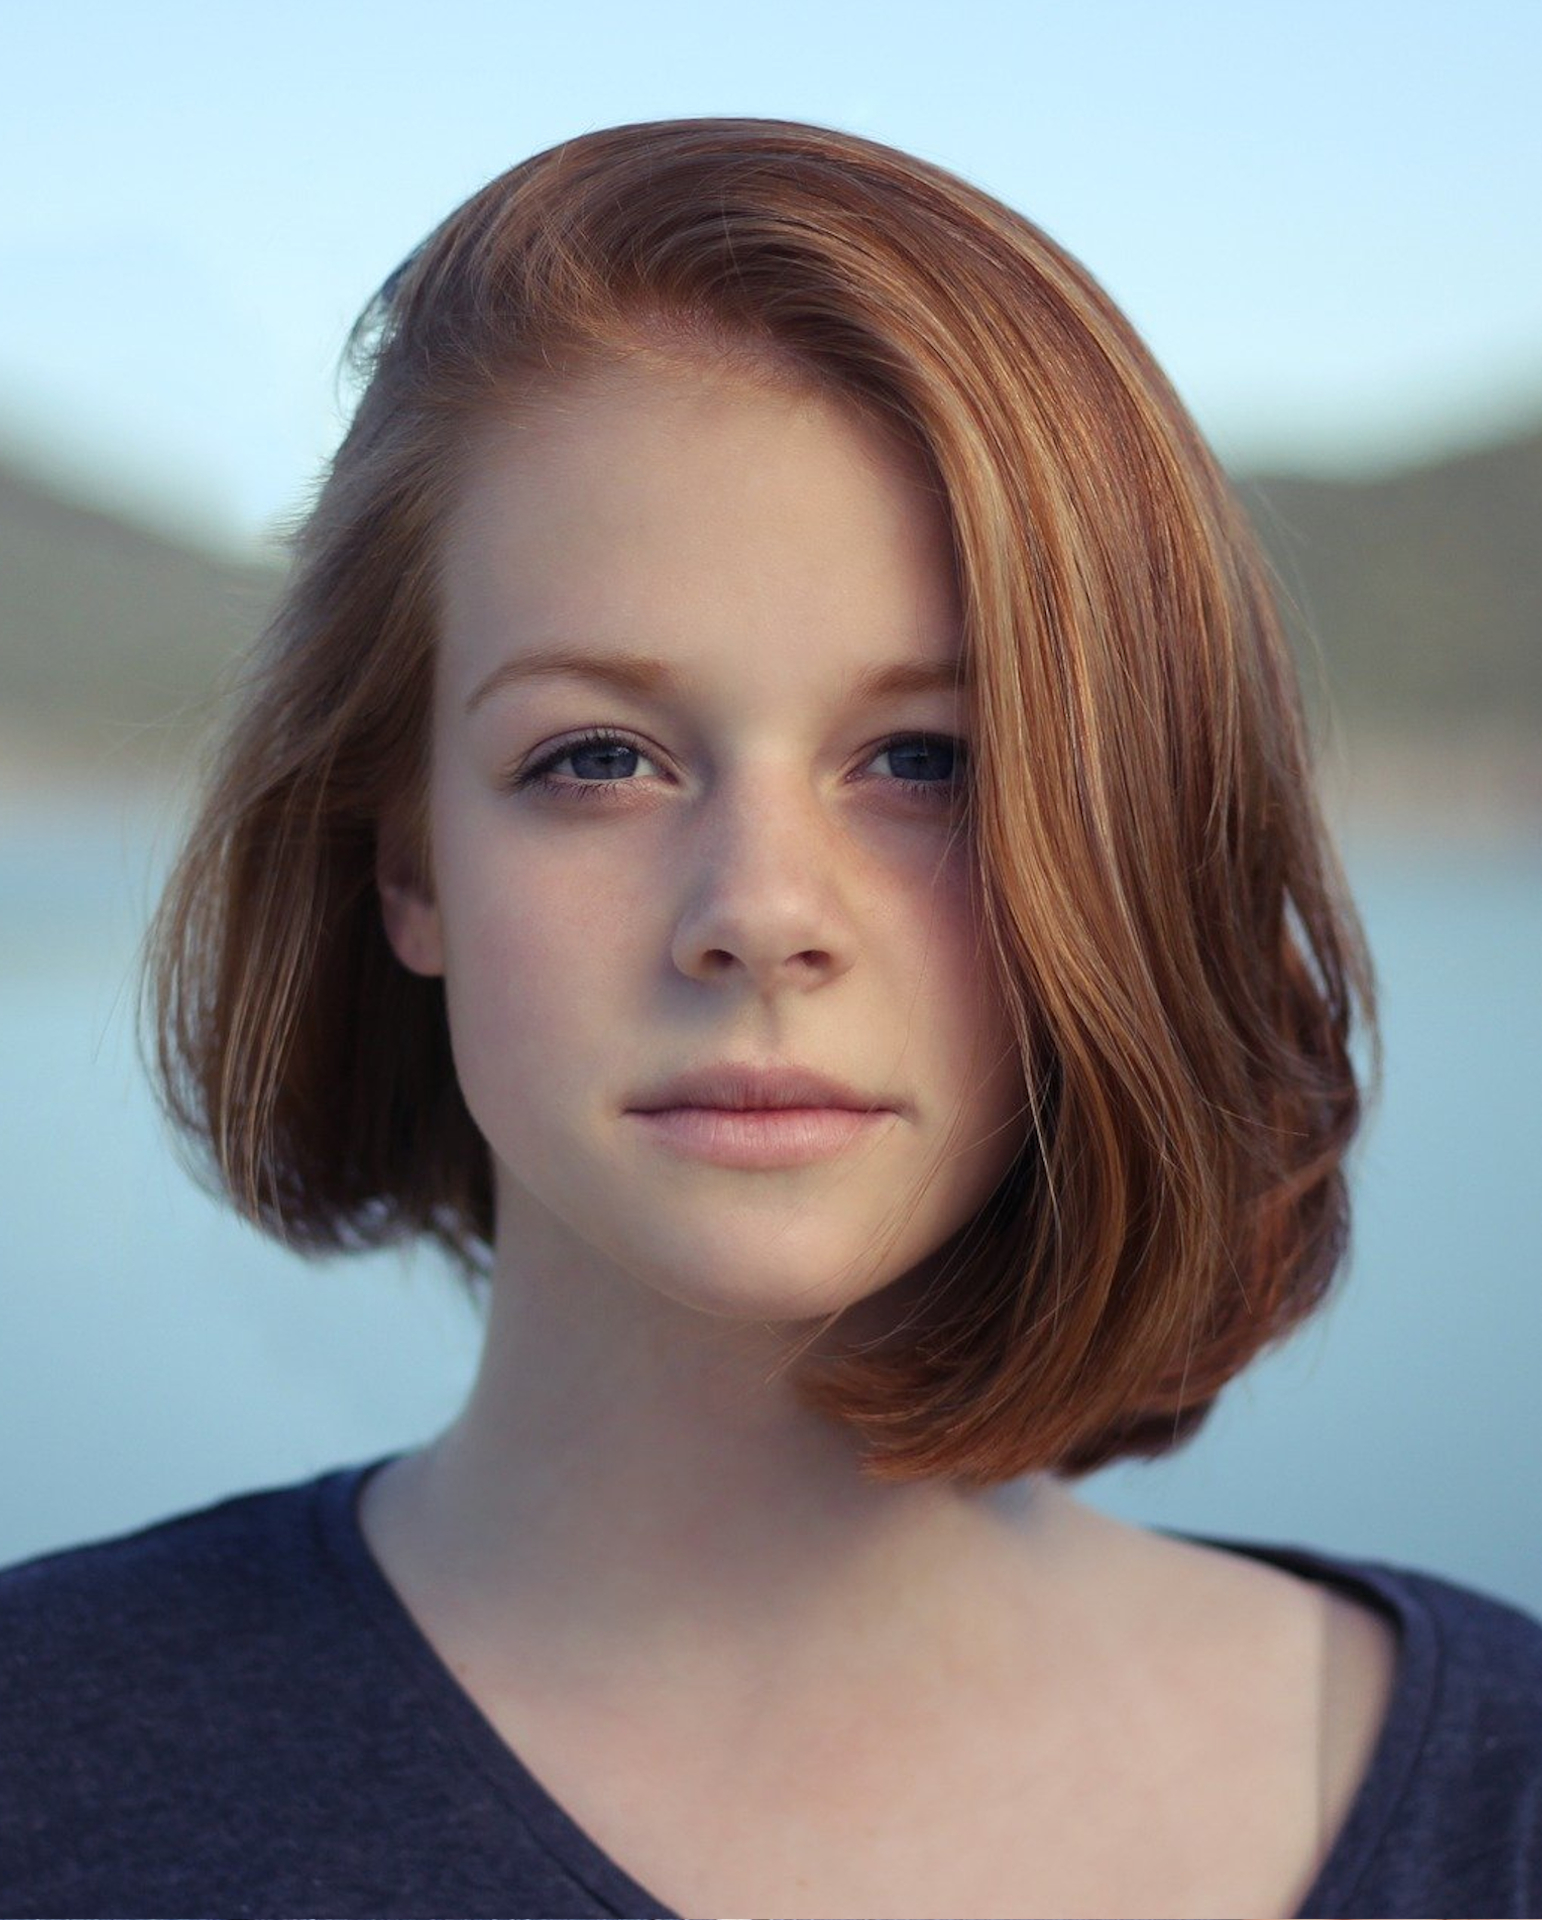
\includegraphics[scale=0.04]{figuras/personas/girl-919048_1920.jpg}
Fonte: Pixabay\tablefootnote{https://pixabay.com/photos/girl-portrait-hairstyle-redhead-919048/}
\end{center} 

&

\textbf{Nome: }  Natália Figueiredo

\textbf{Idade:} 23 anos

\textbf{Ocupação:} Estudante de Engenharia de Software na UnB - Gama.

\\ \hline


\multicolumn{2}{|c|}{\textbf{Descrição}} \\ \hline
\multicolumn{2}{|p{15cm}|}{
    \begin{tabular}[c]{@{}l@{}}\\
        \textbf{Nunca joguei} jogos para aprendizagem, pois \textbf{não conheci nenhum} que tinha o \\propósito de ensinar o que eu desejava. No caso, seria interessante um jogo o qual eu \\pudesse \textbf{aprender} um conteúdo, \textbf{avaliar} o que aprendi e \textbf{revisá-lo} quando necessário.\\ \textbf{Estou no primeiro semestre} da faculdade, por isto \textbf{não tenho conhecimento} em \\relação a elaboração de design de interfaces. Quando vou sanar alguma dúvida que tenho\\ sobre o conteúdo eu \textbf{pesquiso na internet}, \textbf{assisto vídeo aulas}, utilizo do \textbf{material} \\\textbf{disponibilizado pelo professor}. Além de recorrer aos meus \textbf{colegas e quem estiver} \\\textbf{disposto a ajudar}. \\
        \\
        Acho que um jogo para se estudar teria de ter um \textbf{design simples e atraente}, sendo\\ feito um \textbf{bom uso das fontes e core}s, além de uma \textbf{lógica de jogo} e \textbf{regras fáceis} de\\ entender e de se lembrar. Talvez obter \textbf{recompensas} e ter \textbf{feedbacks} evidenciando meu\\ progresso seria interessante. Ao jogar, espero encontrar \textbf{desafios} não muito difíceis, mas\\ que despertem minha \textbf{atenção}. Seria bom, perceber logo de início que o jogo traz um \\\textbf{conteúdo relevante} e que vou \textbf{conseguir aprendê-lo}. E por fim não seria nada ruim\\ sentir \textbf{prazer} em aprender e ainda me \textbf{divertir}.\\
        \\
    \end{tabular}
} \\ \hline
\end{tabular}
\end{table}